\documentclass[12pt]{article}
\usepackage{graphicx}

\title{MATH4350 \\ Homework Assignment}
\author{Joel Savitz}
\date{Wednesday 8 July 2020}

\begin{document}

\maketitle

\textbf{1. Use the Egyptian method of doubling to find the following products:}
\medskip

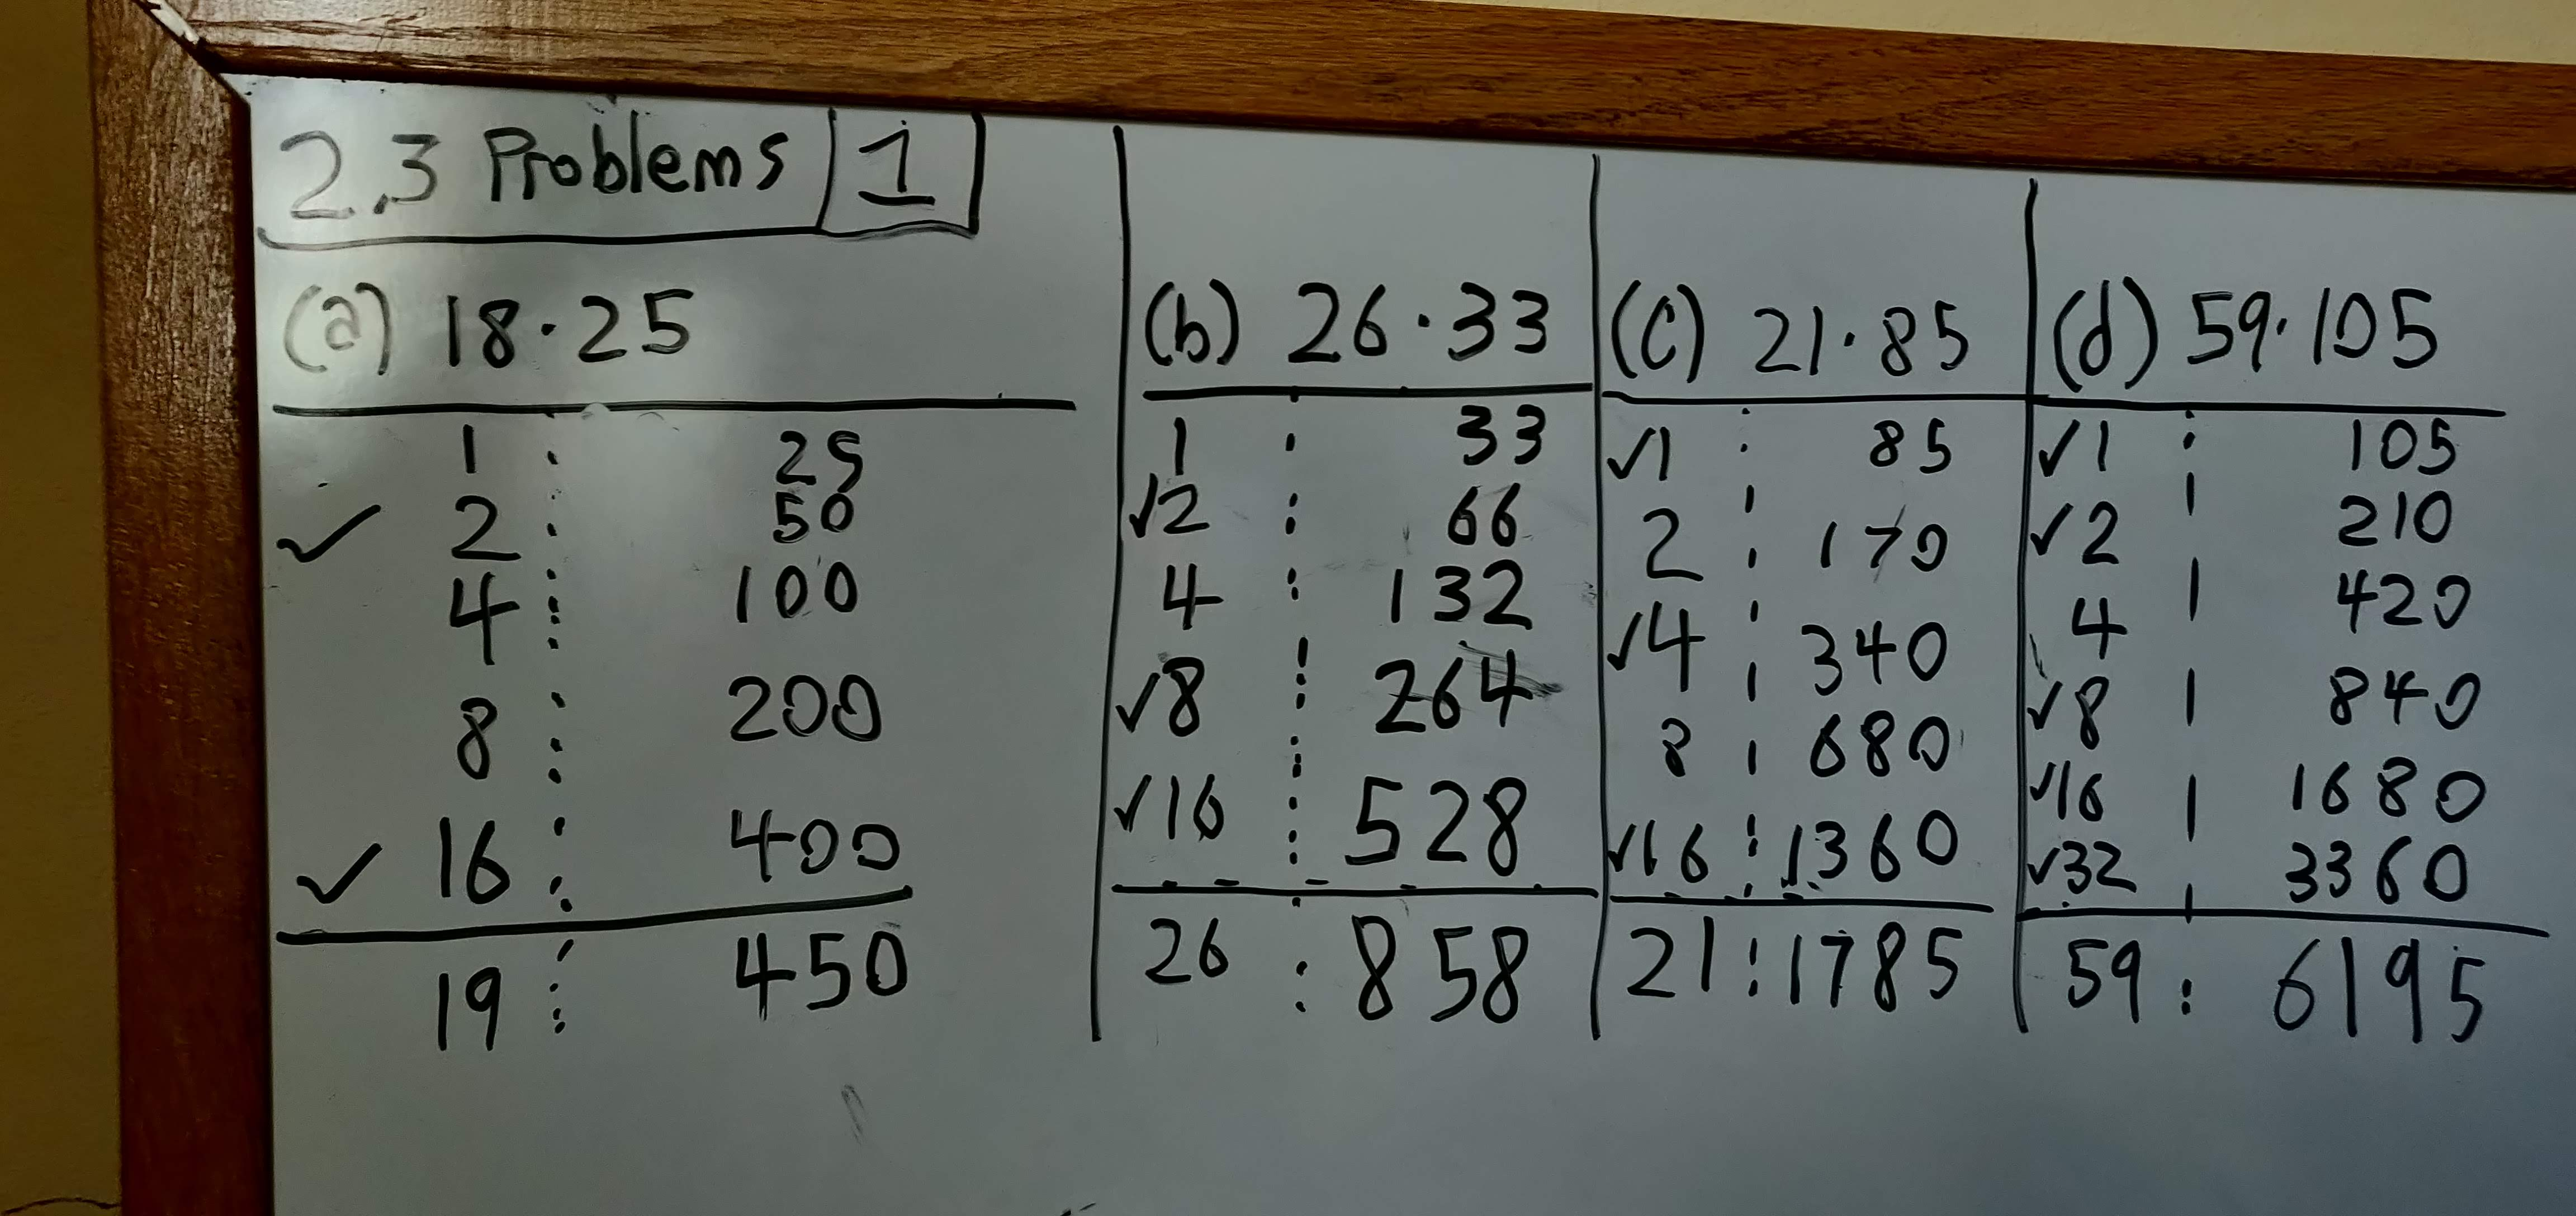
\includegraphics[scale=0.08]{1.jpg}

\pagebreak
\textbf{2. Find, in the Egyptian fashion, the following quotients: }
\medskip

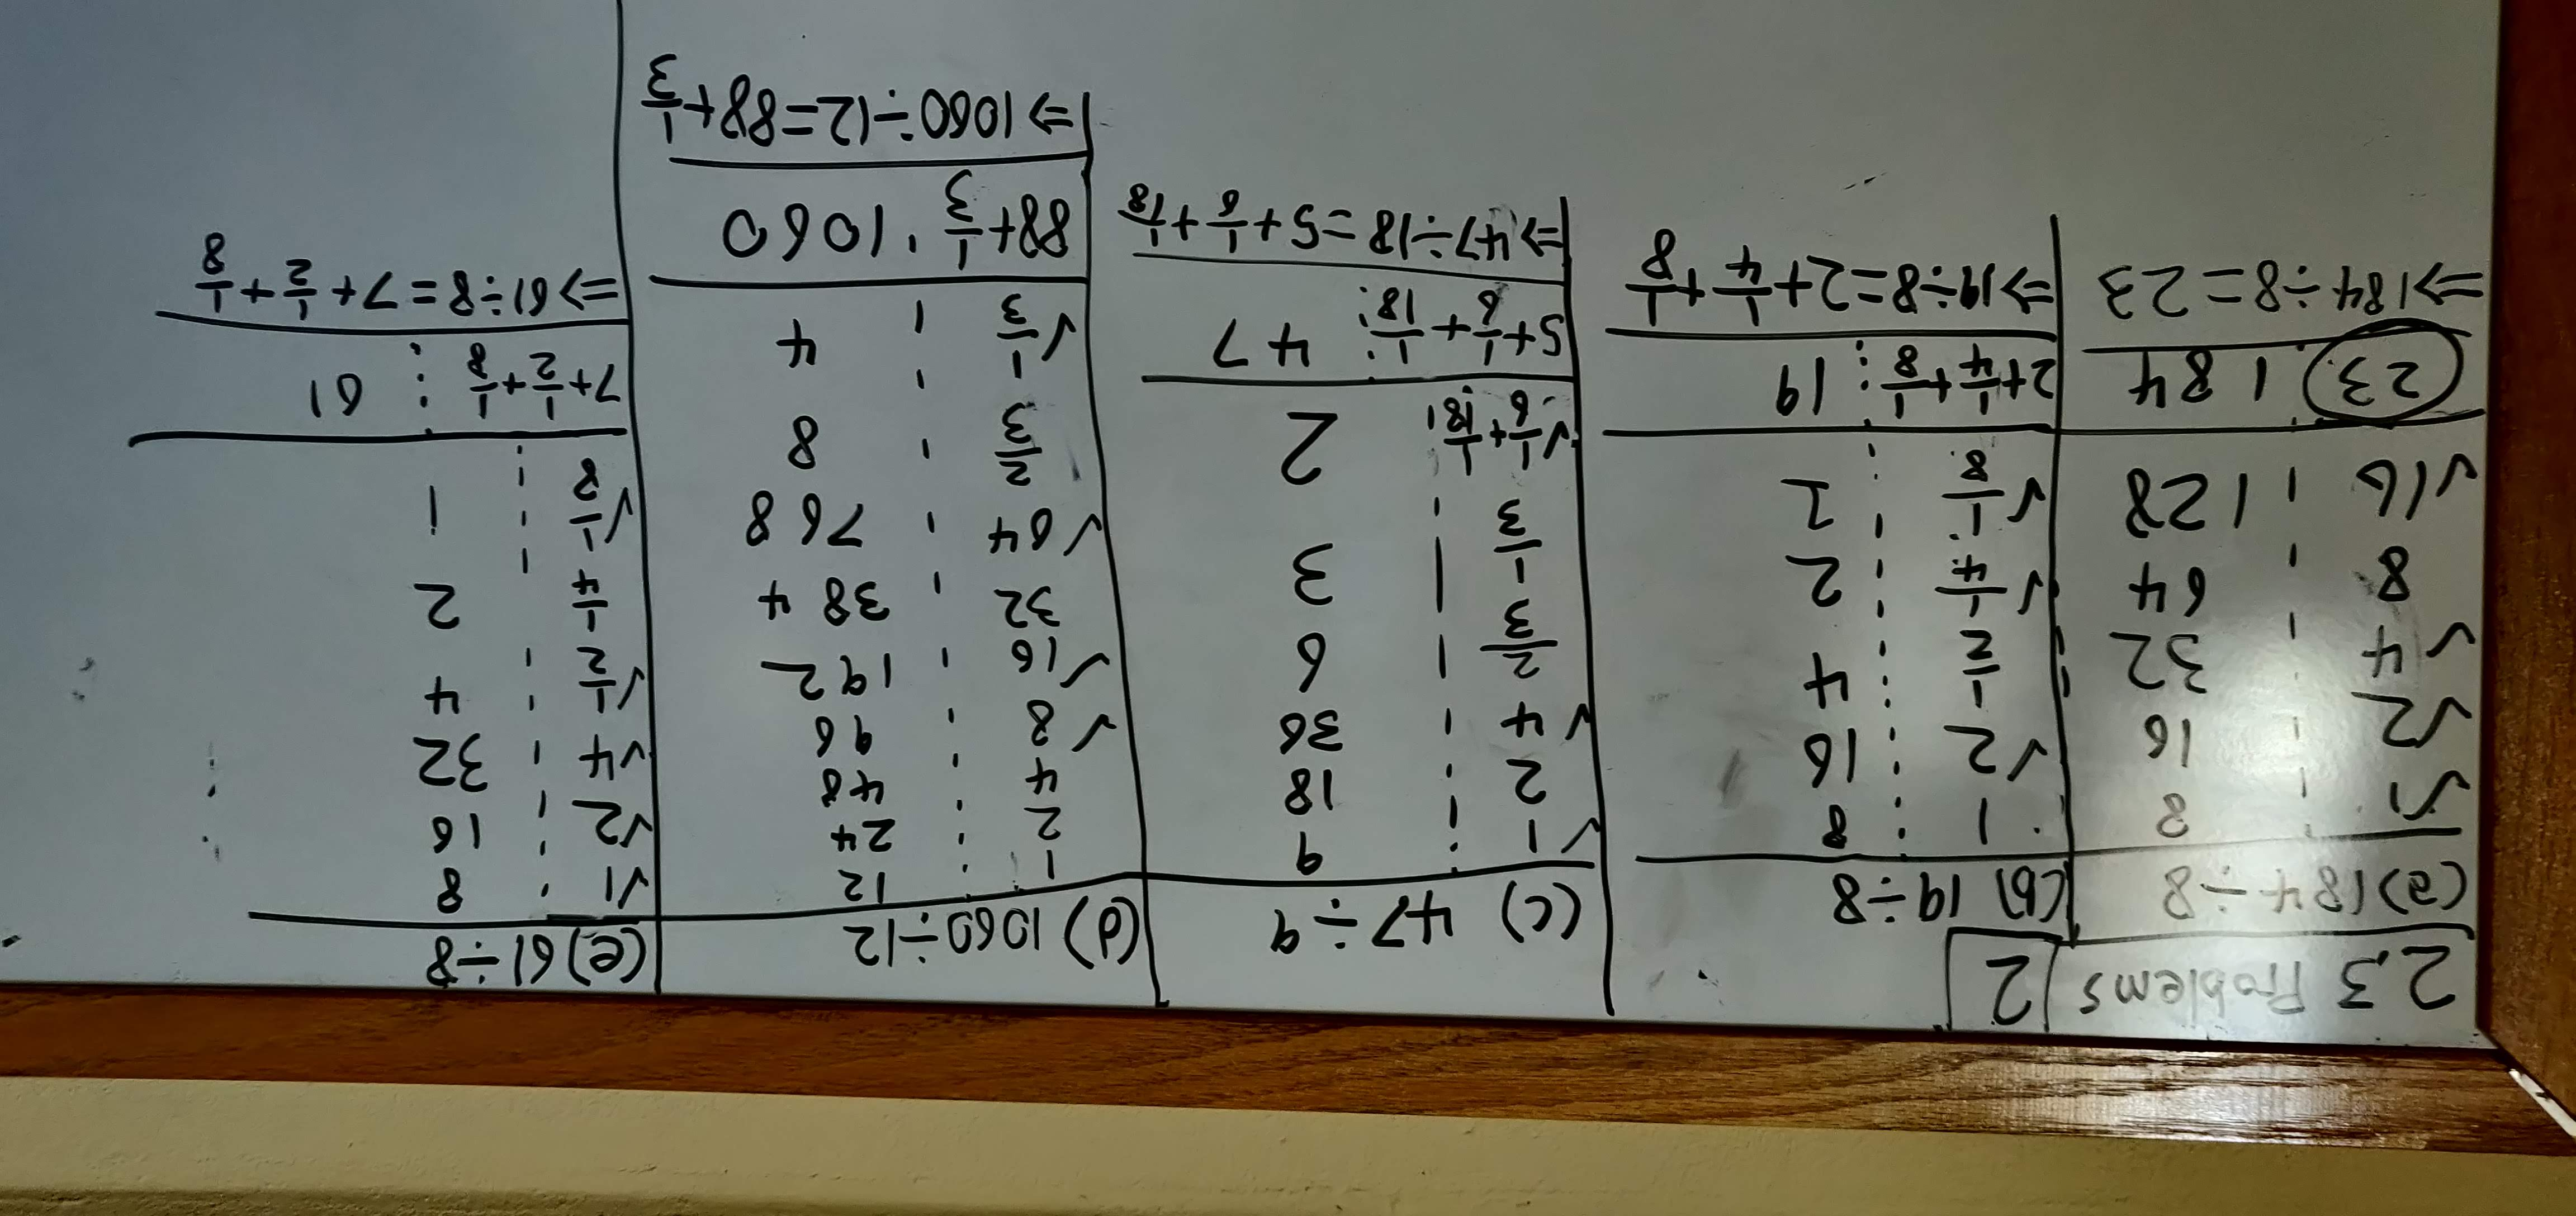
\includegraphics[angle=180, scale=0.08]{2.jpg}

\pagebreak
\textbf{3. Use the Egyptian method of multiplication to calculate the following products: }
\medskip

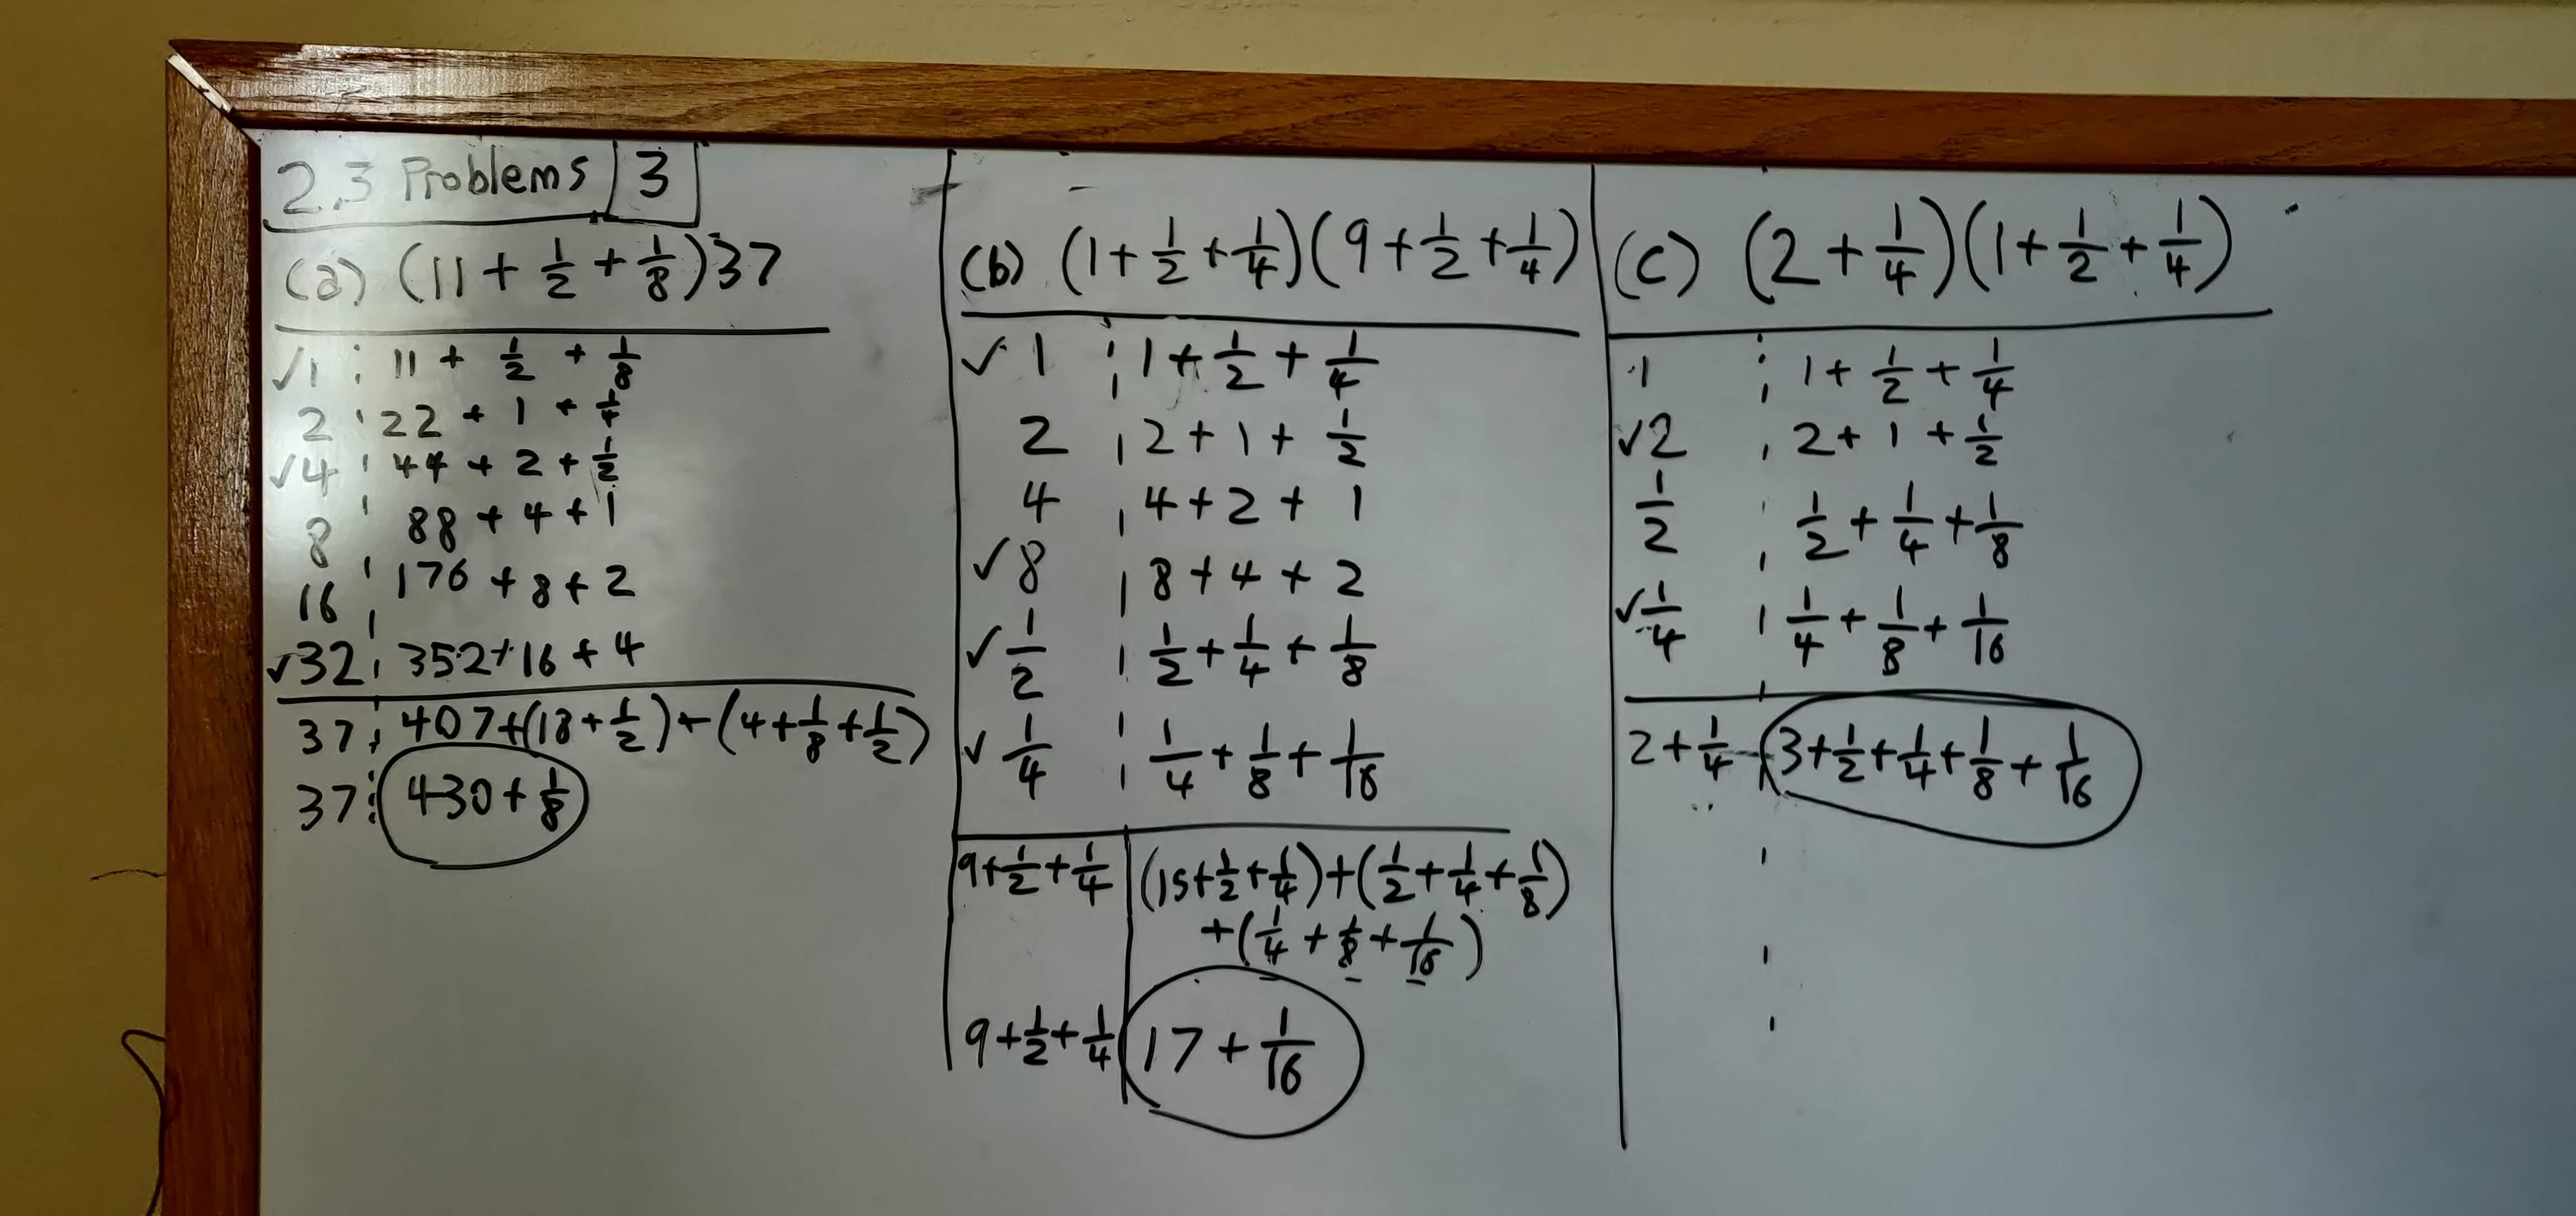
\includegraphics[scale=0.08]{3.jpg}

\pagebreak
\textbf{9. Verify that: $\frac{2}{n} = \frac{1}{n} + \frac{1}{2n} + \frac{1}{3n} + \frac{1}{6n}$
and decompose  $\frac{2}{101}$ accordingly:}
\medskip

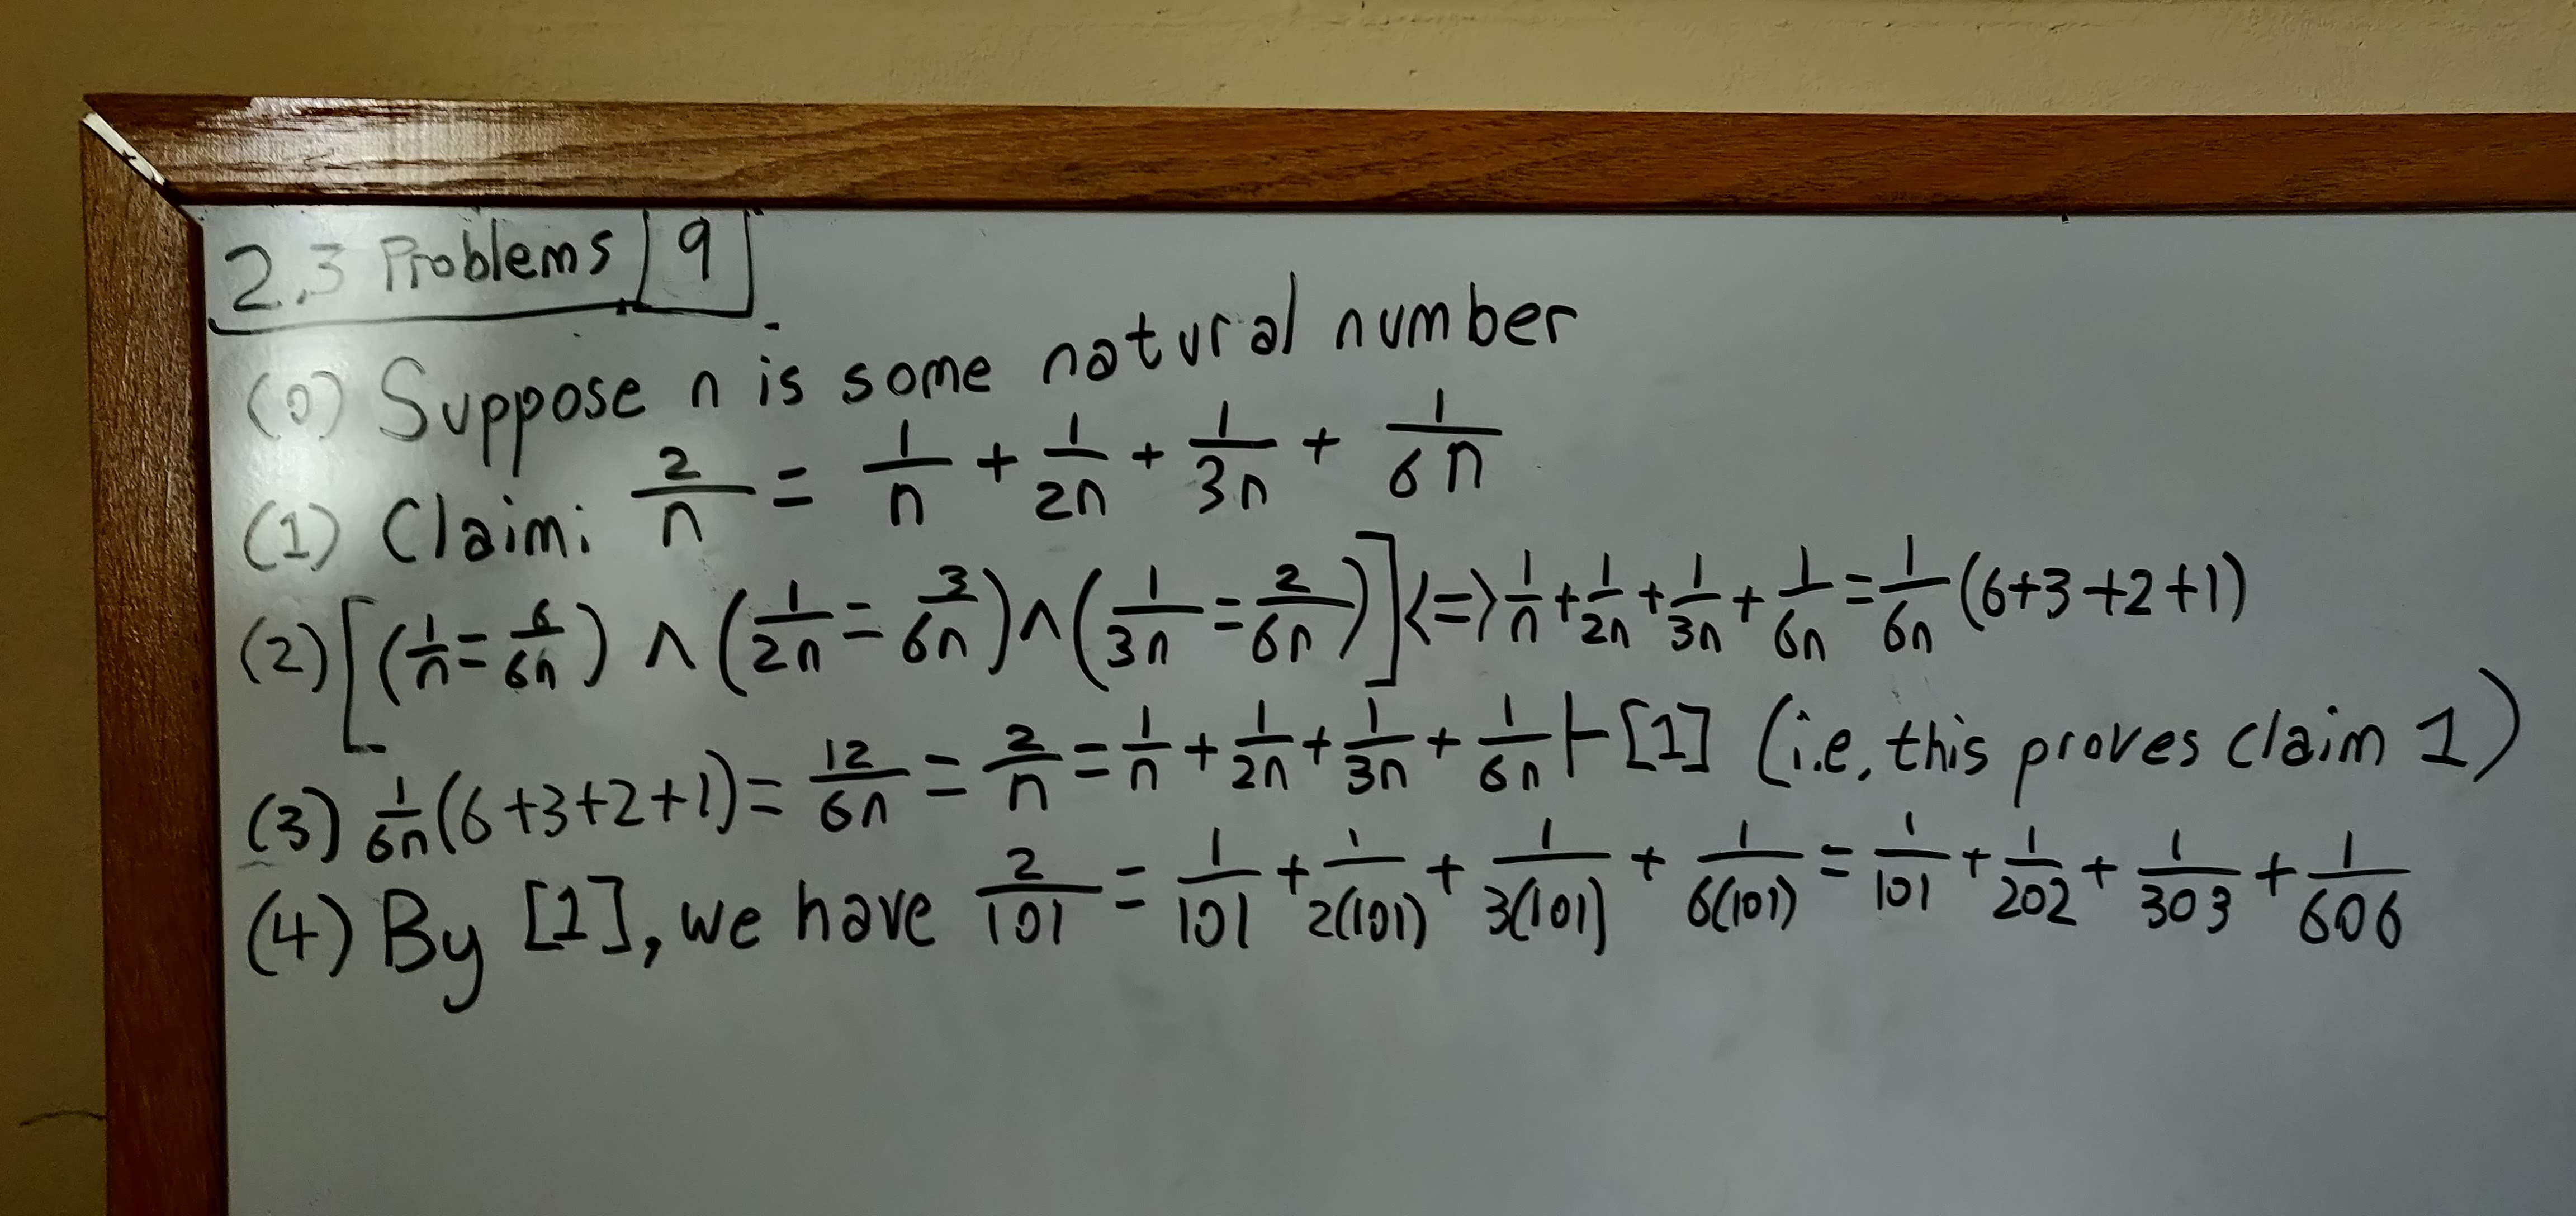
\includegraphics[scale=0.08]{9.jpg}

\end{document}
